\documentclass[border=10pt, multi, tikz]{standalone}
\usepackage{import}
\subimport{../Layers/}{init}
\usetikzlibrary{positioning}
\usetikzlibrary{3d} %for including external image

\def\ConvColor{rgb:yellow,5;red,2.5;white,5}
\def\ConvReluColor{rgb:yellow,5;red,5;white,5}
\def\PoolColor{rgb:red,1;black,0.3}
\def\UnpoolColor{rgb:blue,2;green,1;black,0.3}
\def\FcColor{rgb:blue,5;red,2.5;white,5}
\def\FcReluColor{rgb:blue,5;red,5;white,4}
\def\SoftmaxColor{rgb:magenta,5;black,7}
\def\SumColor{rgb:blue,5;green,15}

\newcommand{\copymidarrow}{\tikz \draw[-Stealth,line width=0.8mm,draw={rgb:blue,4;red,1;green,1;black,3}] (-0.3,0) -- ++(0.3,0);}

\begin{document}
\begin{tikzpicture}
\tikzstyle{connection}=[ultra thick,every node/.style={sloped,allow upside down},draw=\edgecolor,opacity=0.7]
\tikzstyle{copyconnection}=[ultra thick,every node/.style={sloped,allow upside down},draw={rgb:blue,4;red,1;green,1;black,3},opacity=0.7]

\node[canvas is zy plane at x=0] (in_ax) at (0, 4, 0) {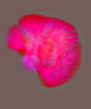
\includegraphics[width=3cm,height=3cm]{ax.png}};

\node[canvas is zy plane at x=0] (in_front) at (0, 0, 0) {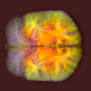
\includegraphics[width=3cm,height=3cm]{front.png}};

\node[canvas is zy plane at x=0] (in_sag) at (0, -4, 0) {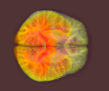
\includegraphics[width=3cm,height=3cm]{sag.png}};

\pic[shift={(2, 0, 0)}] at (in_ax) {
    Box={
        name=conv_ax,
        caption=,
        xlabel={ 1024, },
        zlabel=1,
        fill=\ConvColor,
        height=20,
        width=8,
        depth=20
    }
};

\pic[shift={(2, 0, 0)}] at (in_front) {
    Box={
        name=conv_front,
        caption=,
        xlabel={ 1024, },
        zlabel=1,
        fill=\ConvColor,
        height=20,
        width=8,
        depth=20
    }
};

\pic[shift={(2, 0, 0)}] at (in_sag) {
    Box={
        name=conv_sag,
        caption=,
        xlabel={ 1024, },
        zlabel=1,
        fill=\ConvColor,
        height=20,
        width=8,
        depth=20
    }
};

\node [above=2pt, opacity=1] at (conv_ax-north) {\textbf{ConvNeXt Ax}};
\node [above=2pt, opacity=1] at (conv_front-north) {\textbf{ConvNeXt Front}};
\node [above=2pt, opacity=1] at (conv_sag-north) {\textbf{ConvNeXt Sag}};



\draw [connection]  (in_ax) -- node {\midarrow} (conv_ax-west);

\draw [connection]  (in_front) -- node {\midarrow} (conv_front-west);

\draw [connection]  (in_sag) -- node {\midarrow} (conv_sag-west);

\pic[shift={(2, 0, 0)}] at (conv_front-east) {
    Box={
        name=stack_kv,
        caption=Stack (KV),
        xlabel={ 3, },
        zlabel=1024,
        fill=\ConvColor,
        height=20,
        width=2,
        depth=20
    }
};

\draw [connection]  (conv_ax-east) -- node {\midarrow} (stack_kv-west);

\draw [connection]  (conv_front-east) -- node {\midarrow} (stack_kv-west);

\draw [connection]  (conv_sag-east) -- node {\midarrow} (stack_kv-west);

\pic[shift={(3, 0, 0)}] at (conv_ax-east) {
    Box={
        name=mha_ax,
        caption=,
        xlabel={" ","dummy"},
        zlabel=1024,
        fill=\FcColor,
        height=20,
        width=2,
        depth=20
    }
};

\pic[shift={(3, 0, 0)}] at (conv_front-east) {
    Box={
        name=mha_front,
        caption=,
        xlabel={" ","dummy"},
        zlabel=1024,
        fill=\FcColor,
        height=20,
        width=2,
        depth=20
    }
};

\pic[shift={(3, 0, 0)}] at (conv_sag-east) {
    Box={
        name=mha_sag,
        caption=,
        xlabel={" ","dummy"},
        zlabel=1024,
        fill=\FcColor,
        height=20,
        width=2,
        depth=20
    }
};

\node [above=2pt, opacity=1] at (mha_ax-north) {\textbf{Multi-Head attention}};
\node [above=2pt, opacity=1] at (mha_front-north) {\textbf{Multi-Head attention}};
\node [above=2pt, opacity=1] at (mha_sag-north) {\textbf{Multi-Head attention}};

\draw [connection]  (conv_ax-east) -- node {\midarrow} (mha_ax-west);

\draw [connection]  (conv_front-east) -- node {\midarrow} (mha_front-west);

\draw [connection]  (conv_sag-east) -- node {\midarrow} (mha_sag-west);

\draw [connection]  (stack_kv-east) -- node {\midarrow} (mha_ax-west);

\draw [connection]  (stack_kv-east) -- node {\midarrow} (mha_front-west);

\draw [connection]  (stack_kv-east) -- node {\midarrow} (mha_sag-west);

\pic[shift={(2, 0, 0)}] at (mha_front-east) {
    Box={
        name=stack_attn,
        caption=Stack (Attn),
        xlabel={ 3, },
        zlabel=1024,
        fill=\ConvColor,
        height=20,
        width=2,
        depth=20
    }
};

\draw [connection]  (mha_ax-east) -- node {\midarrow} (stack_attn-west);

\draw [connection]  (mha_front-east) -- node {\midarrow} (stack_attn-west);

\draw [connection]  (mha_sag-east) -- node {\midarrow} (stack_attn-west);

\pic[shift={(2, 0, 0)}] at (stack_attn-east) {
    Ball={
        name=fusion,
        fill=\SumColor,
        opacity=0.6,
        radius=3,
        logo=$\sum$
    }
};

\draw [connection]  (stack_attn-east) -- node {\midarrow} (fusion-west);

\pic[shift={(3, 0, 0)}] at (fusion-east) {
    Box={
        name=fc1,
        caption=Linear + ReLU,
        xlabel={" ","dummy"},
        zlabel=1024,
        fill=\FcColor,
        height=15,
        width=2,
        depth=15
    }
};

\draw [connection]  (fusion-east) -- node {\midarrow} (fc1-west);

\pic[shift={(3, 0, 0)}] at (fc1-east) {
    Box={
        name=fc2,
        caption=Linear,
        xlabel={" ","dummy"},
        zlabel=64,
        fill=\FcColor,
        height=15,
        width=2,
        depth=15
    }
};

\draw [connection]  (fc1-east) -- node {\midarrow} (fc2-west);

\pic[shift={(3, 0, 0)}] at (fc2-east) {
    Box={
        name=soft1,
        caption=,
        xlabel={" ","dummy"},
        zlabel=6,
        fill=\SoftmaxColor,
        opacity=0.8,
        height=8,
        width=1,
        depth=1
    }
};

\node [below=8pt, opacity=1] at (soft1-south) {\textbf{Softmax}};

\draw [connection]  (fc2-east) -- node {\midarrow} (soft1-west);

\end{tikzpicture}
\end{document}
